% !TEX TS-program = pdflatex
% !TEX encoding = UTF-8 Unicode

% This is a simple template for a LaTeX document using the "article" class.
% See "book", "report", "letter" for other types of document.

\documentclass[11pt]{article} % use larger type; default would be 10pt

\usepackage[utf8]{inputenc} % set input encoding (not needed with XeLaTeX)

%%% Examples of Article customizations
% These packages are optional, depending whether you want the features they provide.
% See the LaTeX Companion or other references for full information.

%%% PAGE DIMENSIONS
\usepackage{geometry} % to change the page dimensions
\geometry{a4paper} % or letterpaper (US) or a5paper or....
% \geometry{margin=2in} % for example, change the margins to 2 inches all round
% \geometry{landscape} % set up the page for landscape
%   read geometry.pdf for detailed page layout information

\usepackage{graphicx} % support the \includegraphics command and options

% \usepackage[parfill]{parskip} % Activate to begin paragraphs with an empty line rather than an indent

%%% PACKAGES
\usepackage{booktabs} % for much better looking tables
\usepackage{array} % for better arrays (eg matrices) in maths
\usepackage{paralist} % very flexible & customizable lists (eg. enumerate/itemize, etc.)
\usepackage{verbatim} % adds environment for commenting out blocks of text & for better verbatim
\usepackage{subfig} % make it possible to include more than one captioned figure/table in a single float
% These packages are all incorporated in the memoir class to one degree or another...

%%% HEADERS & FOOTERS
\usepackage{fancyhdr} % This should be set AFTER setting up the page geometry
\pagestyle{fancy} % options: empty , plain , fancy
\renewcommand{\headrulewidth}{0pt} % customise the layout...
\lhead{}\chead{}\rhead{}
\lfoot{}\cfoot{\thepage}\rfoot{}

%%% SECTION TITLE APPEARANCE
\usepackage{sectsty}
\allsectionsfont{\sffamily\mdseries\upshape} % (See the fntguide.pdf for font help)
% (This matches ConTeXt defaults)

%%% ToC (table of contents) APPEARANCE
\usepackage[nottoc,notlof,notlot]{tocbibind} % Put the bibliography in the ToC
\usepackage[titles,subfigure]{tocloft} % Alter the style of the Table of Contents
\renewcommand{\cftsecfont}{\rmfamily\mdseries\upshape}
\renewcommand{\cftsecpagefont}{\rmfamily\mdseries\upshape} % No bold!

% MATH
\usepackage{graphicx}
\usepackage{subfig}

\usepackage{mathtools}
\usepackage{float}
\usepackage{listings}
%%% END Article customizations

%%% The "real" document content comes below...

\title{Numerical Optimization - Handin 2}
\author{Martin Simon Haugaard - CDL966}
%\date{} % Activate to display a given date or no date (if empty),
         % otherwise the current date is printed 

\begin{document}
\maketitle
\section*{2.6}
Examine the statement that \textit{All isolated local minimizers are strict}. This basicly is the same as the logical statement that
\begin{gather*}
\text{'isolated local minimizers' $\implies$ 'local minimizers are strict'}
\end{gather*}
The contrapositive statement will then be
\begin{gather*}
\text{'local minimizers are not strict' $\implies$ 'local minimizers are not isolated'}
\end{gather*}
Examining this last statement, if a local minimizer, $x^*$, is to be not strict, there must be other minimizers, $x$, in the same neighborhood $\mathcal{N}$ which are equal or lower than $x^*$, meaning that $f(x^*) \geq f(x)$ for $x \in \mathcal{N}$.

Now since there are multiple minimizers in the neighborhood, the local minimizers are not isolated. Proving that the contrapositive statement holds true, which in turn proofs our initial statement.

\section*{2.8}
%convex
%show that the set of global minimizers of f is a convex set
Imagine there's a function which will give all the global minimizers, such a function will have to uphold the rule, that for any two points, $x$ and $y$ within its domain $\mathcal{S}$
\begin{gather}
\label{convex:1}
f(\alpha x + (1 - \alpha) y ) \leq \alpha f(x)  + (1 - \alpha) f(y), \text{for all  } \alpha \in [0, 1].
\end{gather}
$\mathcal{S}$ being the set of global minimizers, any point $x$ and $y$ will, when computed in $f$ result in the same value (the global minimum). Thus (\ref{convex:1}) can be reduced to
\begin{gather}
\label{convex:2}
f(\alpha x(1-\alpha)y) = \text{Global Minimum}
\end{gather}
From (\ref{convex:2}) it's evident that any values, $x$ or $y$ will result in being a global minimum. Proving that $\mathcal{S}$ is a convex set,  as any two points from the set will result in (\ref{convex:2}) to remain within the set.
\section*{2.9}
It's stated in the book, that for $p_k$ to be a downhill direction, the angle $\Theta_k$ between $p_k$ and  $\Theta f_k$ has $\cos \Theta_k < 0$, so that
\begin{gather}
p_k^T \nabla f_k = \lVert p_k \rVert \lVert \nabla f_k \rVert \cos \Theta_k < 0
\end{gather}
Calculating $\nabla f$
\begin{gather*}
\nabla f = \begin{bmatrix}2(x_1 + x_2^2) \\ 4x_2 (x_1 + x_2^2 \end{bmatrix}
\end{gather*}
It's possible to fill in the values for $p_k ^ T$ and $\nabla f_k$
\begin{gather*}
\begin{pmatrix}-1, 1\end{pmatrix}\begin{pmatrix}2 \\ 0\end{pmatrix} = -2
\end{gather*}
Since $\lVert p_k \rVert \lVert \nabla f_k \rVert$ is always positive, for the result to be $-2$, $\cos \Theta_k < 0$
meaning $p_k$ is a descent direction.
\\
~
\\
Next for solving
\begin{gather}
\label{2.9.0}
f(x_1, x_2) = (x_1 + x_2^2)^2
\end{gather}
for problem $(2.10)$:
\begin{gather}
\label{2.9.1}
f(x_k + \alpha p_k)
\end{gather}
if $p_k = \begin{pmatrix}-1 \\ 1\end{pmatrix}$ and $x_k = \begin{pmatrix}1 \\ 0\end{pmatrix}$ then (\ref{2.9.1}) becomes
\begin{gather*}
f(x_k + \alpha p_k)  = f(\begin{pmatrix}-1\alpha + 1\\ \alpha + 0\end{pmatrix}
\end{gather*}
And finally using (\ref{2.9.0}) there's
\begin{gather*}
f(x_k + \alpha p_k) = (1-\alpha + \alpha^2)^2
\end{gather*}
Now, to find the global minimizers, the gradient has to be zero:
\begin{gather*}
\frac{\partial f}{\partial \alpha} = 2(2\alpha -1) (\alpha^2 - \alpha +1) = 0
\end{gather*}
For which only $\alpha = \frac{1}{2}$ is the only real solution, being either a local maximum or minimum. To figure out which, the Hessian is examined:

\begin{gather*}
\frac{\partial^2 f}{\partial^2 \alpha} = 12 \alpha ^2 - 12 \alpha + 6 \xrightarrow[]{\alpha = \frac{1}{2}}3-6+6 = 3
\end{gather*}
Since the hessian is positive, $\alpha = \frac{1}{2}$ is indeed the local minimum.
\newpage
\section*{Programming Exercises}
After having implemented the Jacobian calculation for a given Kinematics chain, it's time to evaluate the result it produces:
\begin{gather*}
J=\begin{bmatrix}-0.7071&0&0\\
-1.7071&-1.0000&0\\
0&0&0\end{bmatrix}
\end{gather*}
The Jacobian matrix, $J$, above, is the result of the chain 
which starts in $(0,0,0)$, and has joints in $(0,1.0,0)$, $(-0.7071, 1.7071, 0)$ and ends in $(-1.7071, 1.701, 0)$ (Figure~\ref{fig:chain}). What the Jacobian tells us, is the remainder transformation from a given joint, to the final position of the chain.

Looking at these three columns in the $J$ matrix, the final column is zero since the transformation needed upon the last point to each the end-effect is zero, as $\overrightarrow{e} = \overrightarrow{p_3}$.

\begin{figure}[H]
    \centering
    \includegraphics[width=0.6\textwidth]{ik_inv}
    \caption{The chain plotted}
    \label{fig:chain}
\end{figure}

From P2 the transformation needed is that of moving a distance of $1$ along the X-axis. And finally the transformation needed in $P1$ is in both the X (-1.7071) and Y-axis (0.7071, as negative Y-values indicate an increase in value).

Generally speaking, the Jacobian matrix informs us of the distance, and direction a transformation may be needed in order to arrive at the end-effect. And as such, each column in the matrix should ideally reduce the absolute value of the input, until $(0,0,0)$ is achieved, if this was not the case for my input, and it had for example increasingly large values, the Jacobian would be transforming away from the end-effect.
\newpage
Having re-implemented the Rosenbrock to take a single input of form $z=\begin{bmatrix}x\\y\end{bmatrix}$, as a script called \textit{rosen}, using the following commands:
\begin{lstlisting}[language=matlab]
fun = @rosen;
x0 = [100,100];
options = optimoptions('fminunc','Hessian','on', 'GradObj','on');
[x,g,h] = fminunc(fun,x0,options)
\end{lstlisting}
fminunc gives the following output:
\begin{lstlisting}
x =  1.0000    1.0000
g =  8.9001e-18
h = 1
\end{lstlisting}
Once again confirming that $x=(1.0,1.0)$ is a minimum. Even if the gradient, $g$, is ever so slightly different from zero, it's well within the uncertainty a optimization algorithm may have.

For good measure I also tried with an initial position of $(-100, -100)$, the gradient remains close to zero. While the Hessian changes to 3, which indicated that the slope on one side of the minimum may be stepper than on the other (as the guesses approach from the opposite site).

It's worth nothing that starting the algorithm with a less accurate guess, by default matlab will stop guessing after 200 iterations, making the initial guess matter beyond reducing the time required for matlab to finish processing.
%\section*{Exercise 2.1}
%\label{ex:2.1}
%Gradient $\nabla f(x)$:
%
%\begin{gather}
%\label{lab:gradient}
%\nabla f(x) = \begin{bmatrix} \frac{\partial f}{\partial x_1} \\[6pt] \frac{\partial f}{\partial x_2} \end{bmatrix}
%\end{gather}
%\begin{gather*}
%\frac{\partial f}{\partial x_1} = 100*2(x_2-x_1^2)(-2x_1)+2(1-x_1)(-1) =-400x_1(x_2-x_1^2)-2(1-x_1)
%\\
%\frac{\partial f}{\partial x_2} = 200(x_2-x_1^2)
%\end{gather*}
%Which in (\ref{lab:gradient}) gives:
%\begin{gather*}
%\nabla f(x) = \begin{bmatrix} -400x_1(x_2-x_1^2)-2(1-x_1) \\ 200(x_2-x_1^2) \end{bmatrix}
%\end{gather*}
%
%Hessian $\nabla^2 f(x)$:
%\begin{gather}
%\label{lab:hessian}
%\nabla^2 f(x) = \begin{bmatrix} \frac{\partial^2 f}{\partial x_1^2} & \frac{\partial^2 f}{\partial x_1 \partial x_2} \\[6pt]
%\frac{\partial^2 f}{\partial x_2 \partial x_1} & \frac{\partial^2 f}{\partial x_2^2}
%\end{bmatrix}
%\end{gather}
%\begin{gather*}
%\frac{\partial^2 f}{\partial x_1^2} = -400(x_1(-2x_1)+(x_2-x_1^2)(1)) + 2 = -400(x_2-3x_1^2)+2\\
%\frac{\partial^2 f}{\partial x_1 \partial x_2}  = \frac{\partial^2 f}{\partial x_2 \partial x_1} =-400x_1\\
%\frac{\partial^2 f}{\partial x_2^2} =  200
%\end{gather*}
%Which in (\ref{lab:hessian}) gives:
%\begin{gather*}
%\nabla^2 f(x) = 
%\begin{bmatrix}
%-400(x_2-3x_1^2)+2 & -400x_1 \\
%-400x_1 & 200
%\end{bmatrix}
%\end{gather*}
%For $x^* = (1,1)^T$
%\begin{gather*}
%\nabla f(x^*) = \begin{bmatrix}-400*1(1-1) - 2(1-1) \\ 200(1-1)\end{bmatrix} = \begin{bmatrix}0 \\ 0\end{bmatrix}
%\end{gather*}
%which indicated that $f(x^*)$ is either a local maximum or minimum.
%
%\begin{gather*}
%\nabla^2 f(x) = 
%\begin{bmatrix}
%-400(1-3*1^2)+2 & -400*1 \\
%-400*1 & 200
%\end{bmatrix} = \begin{bmatrix} 802 & -400  \\ -400 & 200 \end{bmatrix}
%\end{gather*}
%From this we can observe that all eigenvalues of the Hessian are positive, and we can also compute that the determinant is positive:
%\begin{gather*} (802 * 200) + (- 400 * -400) = 160400 +160000 = 320400 > 0 \end{gather*}
%Meaning that $f(x^*)$ is indeed a local minimum.
%
%\section*{Exercise 2.2}
%In order to have only one stationary point, the gradient can have only one point where it equals zero.
%Remembering (\ref{lab:gradient})
%\begin{gather*}
%\frac{\partial f}{\partial x_1} = 8+2x_1 \\
%\frac{\partial f}{\partial x_2} = 12-4x_2\\
%\nabla f(x) = \begin{bmatrix} 8+2x_1 \\ 12 - 4x_2 \end{bmatrix} = \begin{bmatrix} 0 \\ 0 \end{bmatrix} \\
%x_1 = -4\\
%x_2 = 3
%\end{gather*}
%When altering the $x_1$ value it results in an increase of value, while altering the $x_2$ results in a decrease of value, meaning the function increases with a different $x_1$ and decreases with a different $x_2$, making the point $(-4, 3)^T$ a saddle point. Figure~\ref{fig:contour} shows a handmade sketch of the saddle point.
%
%\begin{figure}[H]
%    \centering
%    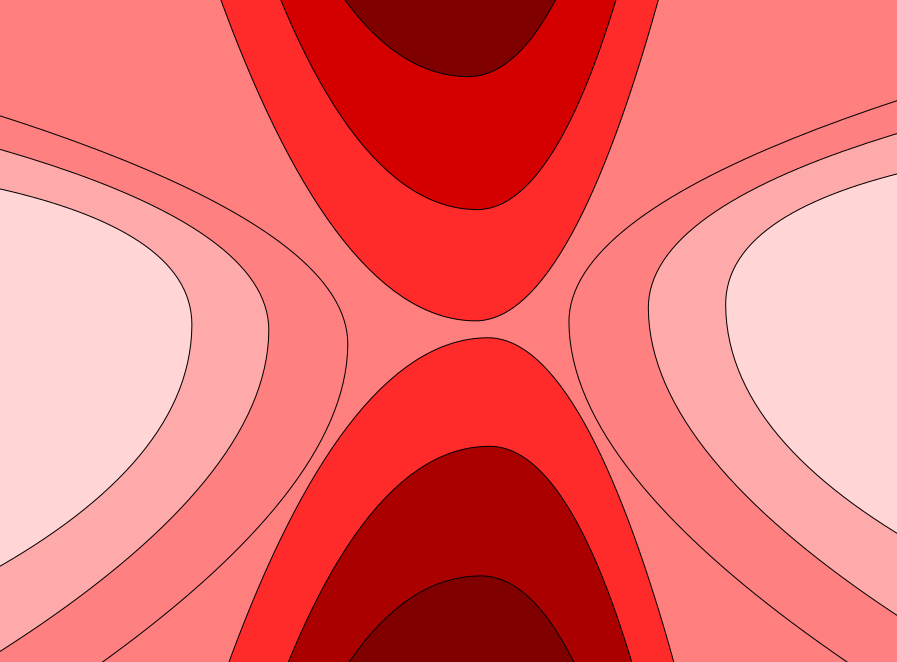
\includegraphics[width=0.4\textwidth]{contur}
%    \caption{Contour sketch of Saddle Point}
%    \label{fig:contour}
%\end{figure}
%
%\section*{Exercise 2.4}
%Omitted due to 5-page limit.
%\section*{Programming}
%\subsection*{Inverse Kinematic}
%After implementing the function in matlab, the following figure (Fig.~\ref{fig:ik1}) is being plotted.
%\begin{figure}[H]
%    \centering
%    \includegraphics[width=0.8\textwidth]{ik}
%    \caption{Inverse Kinematic, starting at (0,0), ending at roughly (-1.7071, 1.7071)}
%    \label{fig:ik1}
%\end{figure}
%Altering the last angle will have no effect, as there's three angles given for three points, but since the first point is always related to the normal space (first plot in Figure~\ref{fig:ik1} is at (0,1), and not at a 45 degree angle), only the first and second given angle will have effect. The last angle will only be relevant for the direction which and future points may be placed.
%
%Figure~\ref{fig:more_ik} shows what happens if the angles are inverted, or if the angles are twice as big.
%
%\begin{figure}[H]
%    \centering
%    \subfloat[Inverted angles]{{\includegraphics[width=0.4\textwidth]{ik_inv} }}%
%    \qquad
%    \subfloat[$\pi/2$ angles]{{\includegraphics[width=0.4\textwidth]{ik_bigger} }}%
%    \caption{Inverse Kinematic with different angles, notice the initial point is unchanged.}%
%    \label{fig:more_ik}%
%\end{figure}
%
%\subsection*{Rosenbrock}
%After having implemented the Rosenbrock function, plotting the graph gives the following figure:
%\begin{figure}[H]
%    \centering
%    \includegraphics[width=0.7\textwidth]{rosen_def}
%    \caption{The Rosenbrock function in effect}
%    \label{fig:rosen_def}
%\end{figure}
%Which, when observed from top down, gives us the desired 'banana':
%\begin{figure}[H]
%    \centering
%    \includegraphics[width=0.7\textwidth]{rosen}
%    \caption{Banana Rosenbrock}
%    \label{fig:banana}
%\end{figure}
%Computing the gradient and Hessian in the minimum $(1,1)$, yields the same result as in Exercise 2.1. 
%
%In $(0,0)$ the gradient becomes $(-2, 0)$ while the Hessian becomes \begin{math}\begin{bmatrix}2 & 0 \\ 0 & 200\end{bmatrix}\end{math} which indicated that it is not a stationary point, which is indeed correct.
%Point $(2,2)$ gives gradient $(1602, -400)$ and Hessian \begin{math}\begin{bmatrix}4002 & -800 \\ -800 & 200\end{bmatrix}\end{math}. 
%
%Depending on where the point is, the values may increase drastically, even if they are relatively close to the stationary point. As the slopes of the plane suddenly become very steep.
\end{document}
